\newpage
\subsubsection{Aufbau (von Nagios)}


Barth schreibt über Nagios: \begin{quote}"`Die große Stärke von Nagios - auch im Vergleich zu anderen Netzwerküberwachungstools - liegt in seinem modularen Aufbau: Der Nagios-Kern enthält keinen einzigen Test, stattdessen verwendet er für Service- und Host-Checks externe Programme, die als \textit{Plugins} bezeichnet werden."' \begin{flushright}\cite{Barth08} S. 25\end{flushright}\end{quote} 

Dieser "`Kern"' beinhaltet das komplette Benachrichtigungssystem mit Kontaktadressen und Benachrichtigungsvorgaben (Zeit, Art, zusätzliche Kriterien), die Hosts- und Servicedefinitionen inklusive deren Gruppierungen und schließlich das Webinterface.
Siehe hierfür auch Abbildung \ref{nagios-kern}.

\begin{figure}[ht]
	\centering
	   \fbox{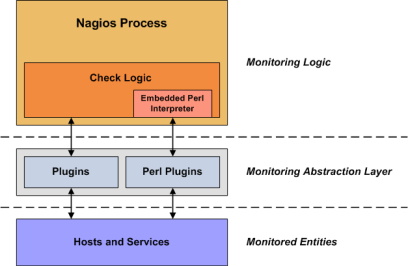
\includegraphics[width=0.85\textwidth]{bilder/nagios-proc.png}}
		\caption{Logische Nagios Struktur\footnote{http://www.nagioswiki.org/w/images/8/81/Plugins.png}}
		\label{nagios-proc}
\end{figure}


Die Plugins werden durch die Servicedefinitionen mit den jeweiligen Hosts verbunden und werden durch eine Befehlskonfigurationsdatei mit ggf. veränderten Parametern durch Nagios aufgerufen.

Das bedeutet, dass die gewünschten Plugins explizit aus dem Nagios Repertoire dem zu überwachendem Computer zugeteilt werden müssen.
Eine beispielhafte Servicedefinition für den Host \textit{iwrpaul.ka.fzk.de} wird in Codelisting \ref{servdef}.

\begin{lstlisting}[captionpos=b, caption=Beispielhafte (Definition) eines Servicechecks, label=servdef, breaklines = true, language=bash]
# Define a service to check the swap disk space
# on the local machine.  Warning if < 20% free, 
# critical if < 10% free space on swap partition.

define service{
 use         generic-service 	;# Name of service template to use
 host_name   iwrpaul.ka.fzk.de 	;# DNS-Name des Hosts
 service_description  Swap Disk Space ;# Beschreibung des Services
 check_command   check_swap!-w 20% -c 10%	;# Angabe des zu verwendenden Plugins mit WARNING (respektiv) CRITICAL Schwellwertparameter
}
\end{lstlisting}

Nagios überprüft in einem festlegbaren / veränderbaren Zeitintervall alle vom Benutzer definierten Host- und Servicechecks und verarbeitet / arbeitet / wertet die Daten / Informationen / Ergebnisse der entsprechenden Plugins aus.

Weiterhin beschreibt Barth die Plugins folgendermaßen:
\begin{quote}"`Jedes Plugin, das bei Host- und Service-Checks zum Einsatz kommt, ist ein eigenes, selbständiges Programm, das sich auch unabhängig von Nagios benutzen lässt."' \begin{flushright}\cite{Barth08} S. 105\end{flushright}\end{quote} 

Daher lassen sich die Parameter eines Plugins folgendermaßen überprüfen:

\begin{figure}[ht]
	\centering
	   \fbox{
\includegraphics[width=0.85\textwidth]{bilder/check-swap-white.png}}
		\caption{Beispielhafte manuelle Ausführung eines Servicechecks}
		\label{check-swap}
\end{figure}

Die Ausgabe des Plugins gibt den Zustand des Services an; in diesem Fall wird kein Schwellwert überschritten, daher die Meldung \pictext{SWAP OK}.

Dabei wird in vier verschiedene Rückgabewerte / Antworten der Plugins unterschieden:

\begin{figure}[ht]
	\centering
	   \fbox{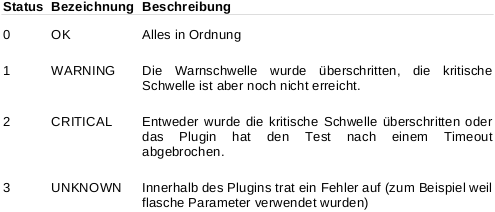
\includegraphics[width=0.85\textwidth]{bilder/nagios-4state-tab.png}}
		\caption{Rückgabewerte für Nagios Plugins}\footnote{Quelle: \cite{Barth08} S. 105f}
		\label{nagios-4states}
\end{figure}

Anhand dieser Werte wertet Nagios gezielt den Status des jeweiligen Objektes (Host oder Service) aus.
Weiterhin gibt es weiche (Soft States) und harte Zustände (Hard States):

\begin{figure}[ht]
	\centering
	   \fbox{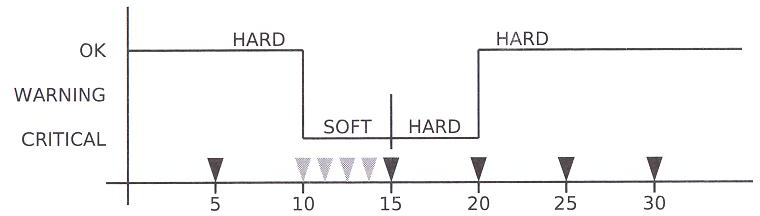
\includegraphics[width=0.85\textwidth]{bilder/hs-states.png}}
		\caption{Beispiel für den zeitlichen Verlauf von Zuständen eines überwachten Dienstes}\footnote{Quelle: \cite{Barth08} S. 95}
		\label{hs-states}
\end{figure}

Ausgehend von einem OK Zustand wird in diesem Beispiel jede fünf Minuten periodisch überprüft, ob sich der Status des übwachten Objektes verändert hat.
Nach zehn Minuten                                                                                                                                                                                             wird ein Umschwenken / Änderung des Zustandes durch das jeweilige Plugin gemeldet\begin{quote}"`; der Zustand wechselt nach CRITICAL, zunächst allerdings als Soft State.
Zu diesem Zeitpunkt löst Nagios noch keine Benachrichtigung aus"'\end{quote}, da es sich um eine Falschmeldung, auch False Positive genannt, handeln kann, aufgrund einer kurzweiligen / kurzfristigen (besseres Wort? peak mäßig) hohen Auslastung des Netzwerkes oder um ein kurzzeitiges Problem, welches sich von alleine wieder normalisiert. (Bspw. Prozessorauslastung)

Nun wird der im Soft State befindliche Service bzw. Host mit einer höheren Frequenz überprüft, damit ein False Positive ausgeschlossen werden kann.
Sollten diese Überprüfungen den vorherigen Zustand bestätigen, verfestigt sich der aktuelle Zustand, man spricht nun von einem Hard State / wechselt der Zustand in den Hard State.
Erst in diesem Moment werden die entsprechenden Kontaktpersonen über den in diesem Beispiel kritischen Zustand benachrichtigt.
Sollte sich der Zustand wieder in den Normalzustand begeben und dieser Zustandsübergang wird von dem (von Nagios ausgeführten) Plugin festgestellt, wird dies an den Nagios Server gemeldet.

Ein Übergang zu dem OK Status wird sofort als Hard State festgelegt / festgehalten / festgesetzt / und führt dadurch zur sofortigen Benachrichtigung durch Nagios.

\begin{itemize}
\item Betroffene OSI Schichten auflisten und erklären
\item Wie werden die Info von Nagios gesammelt und wie gespeichert -> FlapDetection
\item \textbf{Performacedaten???}
\item FLapping \footnote{http://nagios.sourceforge.net/docs/2\_0/flapping.html}
\end{itemize}